%----------------------------------------------------------------------------
\chapter{A lekérdező program}\label{sect:Ellaboration}
%----------------------------------------------------------------------------
\section{Fejlesztés menetének áttekintése}
Első lépésként tehát a bevezetőben megfogalmazott problémák megoldása érdekében, készítettem egy saját magas szintű lekérdező nyelvet az Essbase-hez, mégpedig úgy, hogy a riport valamint az mdx nyelv összetevői alapján megfogalmaztam Xtextben egy metamodellt, amit már az Xtext ezután tud értelmezni, és egy konkrét lekérdezés megírásánál tudja azt validálni.

Majd ezek után az általam újonnan létrehozott nyelvbe, létrehoztam saját lekérdezést, amiben meg lehet nézni a havi kimutatást, költségeket.

Ezután készítettem egy szerkesztőt, amibe a fejlesztők tudnak dolgozni, ehhez egy Eclipse pugint csináltam, beépítve az Xtext nyelvtan elemző programomat. 

A program indítás után áttranszformálja a megírt lekérdezést olyan forráskóddá amit az Essbase értelmezni tud, majd hálózaton keresztül elkéri azt egy objektumba, amivel utána lehet dolgozni. A visszakapott objektumot ezután, a megfelelő parancsal meg lehet jeleníteni, riportolni, egy Latex pdf-be, amit a program generál.

 \begin{figure}[!ht]
\centering
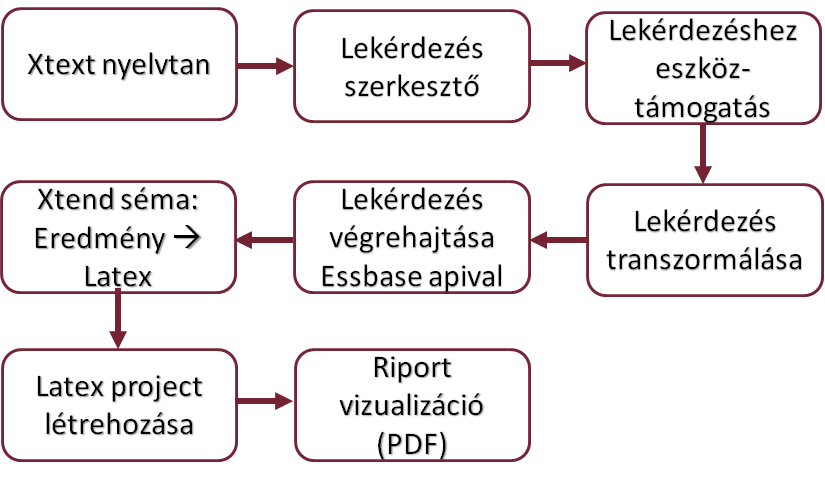
\includegraphics[width=120mm, keepaspectratio]{figures/overview.png}
\caption{A folyamat áttekintése} 
\label{fig:Overview}
\end{figure}

\section{Saját lekérdező nyelv bemutatása}

Először is Xtextbe létrehoztam egy metamodelt, amibe definiáltam a saját riport lekérdezőmbe a valid parancsokat, amik kombinálják az MDX és a Riport parancsok lehetősgéeit, így mindkét nyelv lehetsőségeit lehet használni egy nyelvbe.

Jelenleg elkészült parancsok, amiket a metamodellezőbe már definiáltam.
\begin{itemize}
  \item query: lekérdez az adatbázisból, a paraméterezésének megfelelően,
  gyakorlatilag egy referenciaként lehet használni, amit ezután ki lehet
  riportálni
  \item dim: segítségével létrehozhatunk dimenzió referenciát, amivel ezután
  tudunk hivatkozni más parancsokba
  \item group: segítségével létrehozhatunk group referenciát, amivel ezután
  tudunk hivatkozni más parancsokba
  \item row: definiálhatjuk vele a sorokat, ami majd a kimeneti riportban meg
  fog jelenni, dim vagy group
  \item link: meg lehet adni hogy a kimeneti riportban milyen szintig menjen le
  riport, meg lehet adni dimenziót, csoportot, vagy membert is
  \item reportParameter: speciális paraméter megadására használható, amit a
  fejlesztő környezet felhasznál, és megjelenítést befolyásolja
  \item report: bemenete egy query és futtatáskor a fejlesztő környezet generál
  egy pdf riportot 
\end{itemize}


\section{Validációs módszerek}
Az általam létrehozott új programozási nyelv tehát tudja validálni a megírt kódot már írás közben, egyszerre lehet riportokat és lekérdezéseket fejleszteni, elírások ellen véd a változó hivatkozás.

\section{Futtatás és a riport kimenete}
A megírt lekérdezést Eclipse-be lehet futtatni egy plugin segítségével a képernyőn látható módon:

\begin{figure}[!ht]
\centering
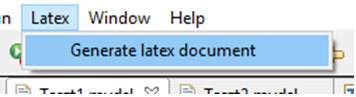
\includegraphics[width=60mm, keepaspectratio]{figures/run.png}
\caption{Riport futtatás Eclipse-ből} 
\label{fig:Overview}
\end{figure}

\newpage
Majd amikor futtatjuk a lekérdezésünket a program generál egy latex projektet, egy Tex fájlal, amibe generálja a program az általunk megírt riport kimenetét:

 \begin{figure}[!ht]
\centering
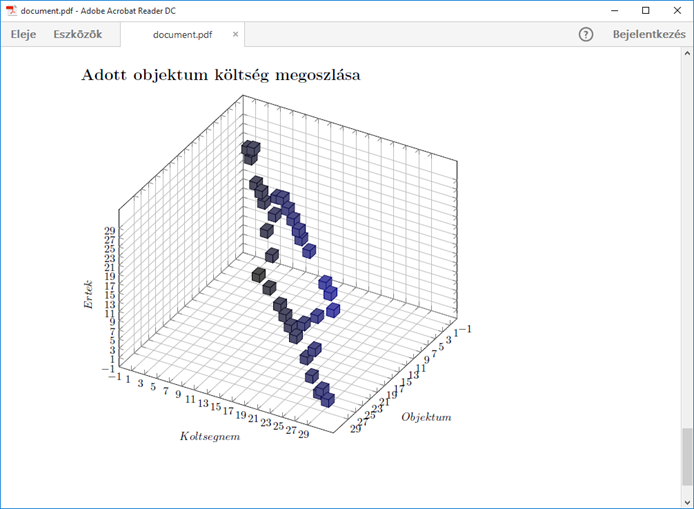
\includegraphics[width=120mm, keepaspectratio]{figures/Report.png}
\caption{Riport diagram példa} 
\label{fig:Overview}
\end{figure}





